\chapter{$\Dsplus$ production in p-Pb collisions at $\s$ = 5.02 TeV}

\section{Measurement of $\Ds/\Dplus$ yield ratios versus multiplicity}
\subsection {Equalisation of the tracklet distribution over z-vertex coordinate}
\label{subsec:zVxtEq}
The multiplicity estimator used for this analysis was based on the number of tracklets reconstructed in the
Silicon Pixel Detector (SPD) within a pseudo-rapidity range of $|\eta| <$ 1. A tracklet in the SPD is obtained by
joining space points on the two SPD layers and it is required to point to the reconstructed primary vertex. 
Events that do not have a reconstructed vertex do not pass the selection criteria, hence
do not contribute to the tracklet distribution.
 In order to check whether there is any variation of the SPD acceptance as a function of the z coordinate
of the reconstructed primary vertex, $\zVtx$, a 2D plot of $\Ntrkl$ against $\zVtx$ was obtained. This is shown in
Fig.~\ref{fig:NtrklVsZ2D} for the periods 16q and 16t, and also for both the FAST and CENT reconstructions.
 The average profiles of the distributions can also be observed superimposed on the plots, and it can be
 observed that there is a dependence on $\zVtx$. The trend of $\averNtrkl$ as a function of $\zVtx$ is only sensitive to SPD acceptance.
 The exclusion of SPD half staves during data acquisition causes a decrease of the number of reconstructed tracklets,
 while the lower $\averNtrkl$ towards large $\zVtx$ is due to finite acceptance of the SPD layers. 
Note that this analysis only considered events passing a cut of $| \zVtx| <$ 10 cm.
 It is important that the distribution of the $\Ntrkl$ vs $\zVtx$ is equalised offline before the selection on the multiplicity, 
in order not to have dependencies on the
 vertex position, which only would arise from acceptance effects depending on time. On this purpose, 
 the average profile of $\Ntrkl$ vs $\zVtx$ was analysed run by run on the full 
 16q, t periods, in order to evaluate the stability of $\averNtrkl$ vs $\zVtx$ as a function of time. Four bunches of runs were indeed
 found with not negligible differences (up to $\sim$10\%) in the $\averNtrkl$ values at positive values of $\zVtx$, as it is shown in Fig.~\ref{fig:FourBunches} (left).
 The equalisation along the $\zVtx$ was hence applied on an event-by-event basis on each of the four bunches of runs separately.
The $\averNtrkl$ value to be used as the absolute reference multiplicity value was defined as the maximum of $\Ntrkl$ as a function of $\zVtx$ 
over the full period, i.e. 29.2 tracklets. The choice of the maximum value is needed to have an unbiased result, 
given that the correction procedure makes use
of a Poissonian extraction for the correction factor $\Delta N = N_{\rm corr}(z) - N_{\rm raw}(z)$. The average $\Ntrkl$ profiles of the four bunches 
after the correction are shown in the right panel of Fig.5\ref{fig:FourBunches}, eventually fitted with a pol1 function in order
to check the flatness of the distribution.


\begin{figure}[h]
\centering
 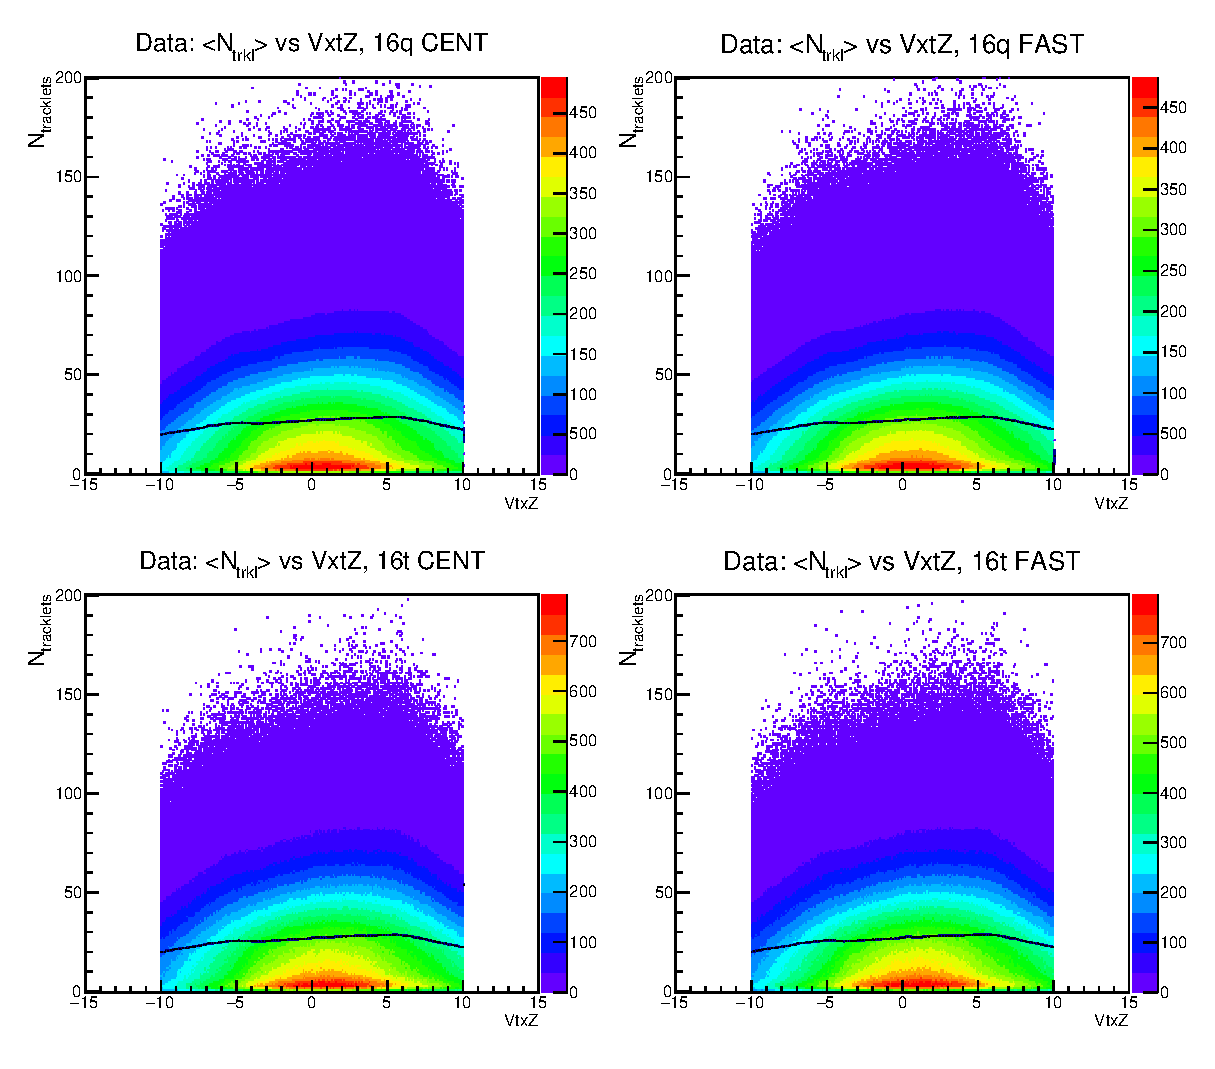
\includegraphics[width=.7\textwidth]{FigCap6/NtrklVsVtxZ_Data.eps}
 \caption{Tracklets distribution as a function of the z-vertex coordinate for the periods 16q and 16t, and for both FAST and CENT reconstructions.}
 \label{fig:NtrklVsZ2D}
\end{figure}


\begin{figure}[h]
\centering
 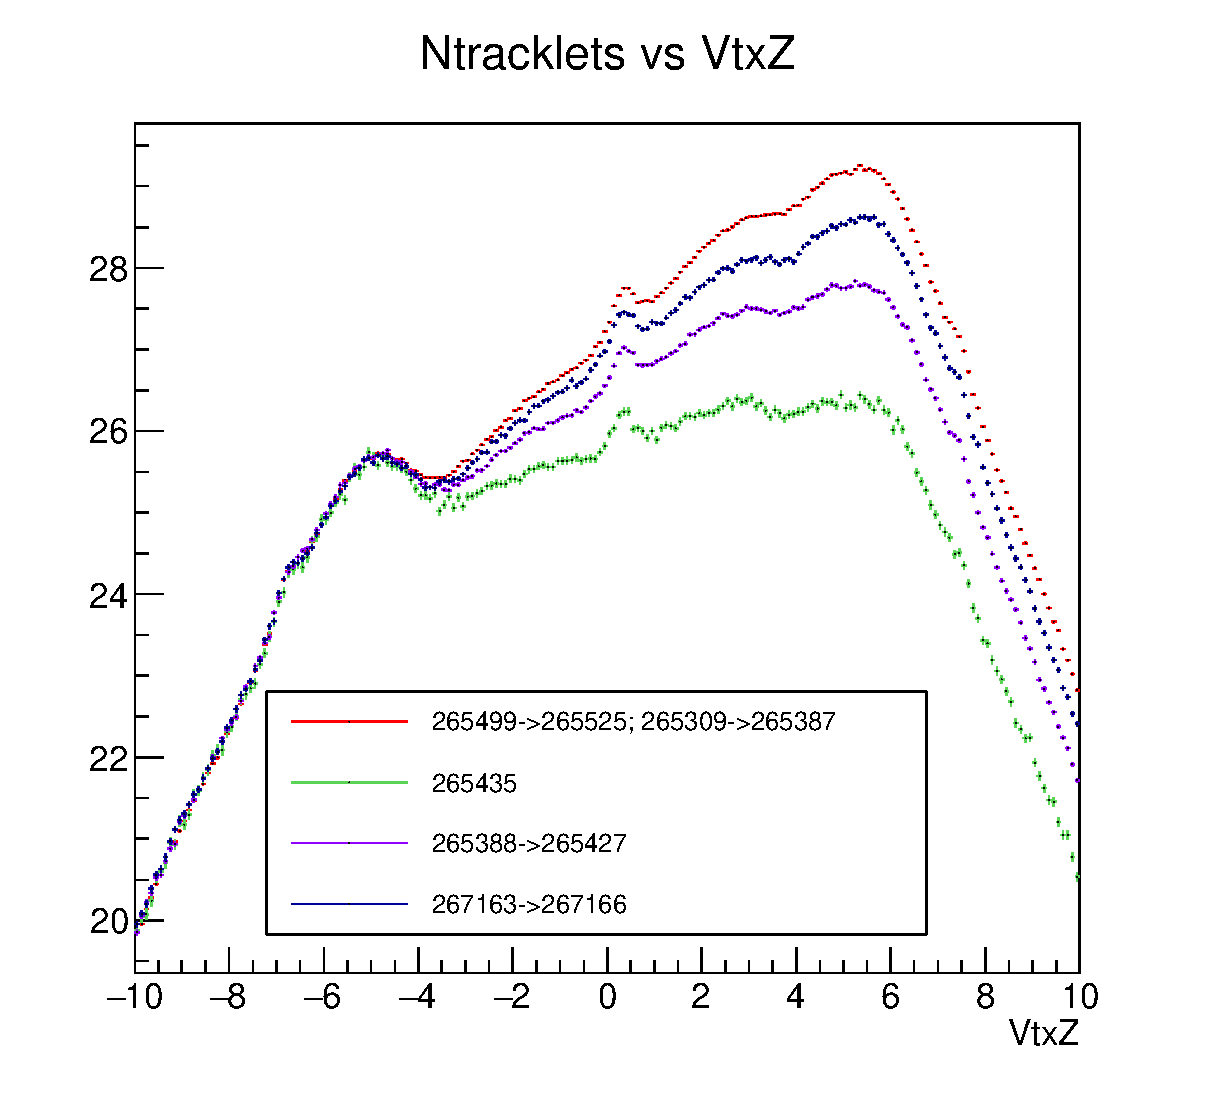
\includegraphics[width=.45\textwidth]{FigCap6/NtrkVsZVtx_FinalWeights.eps}
 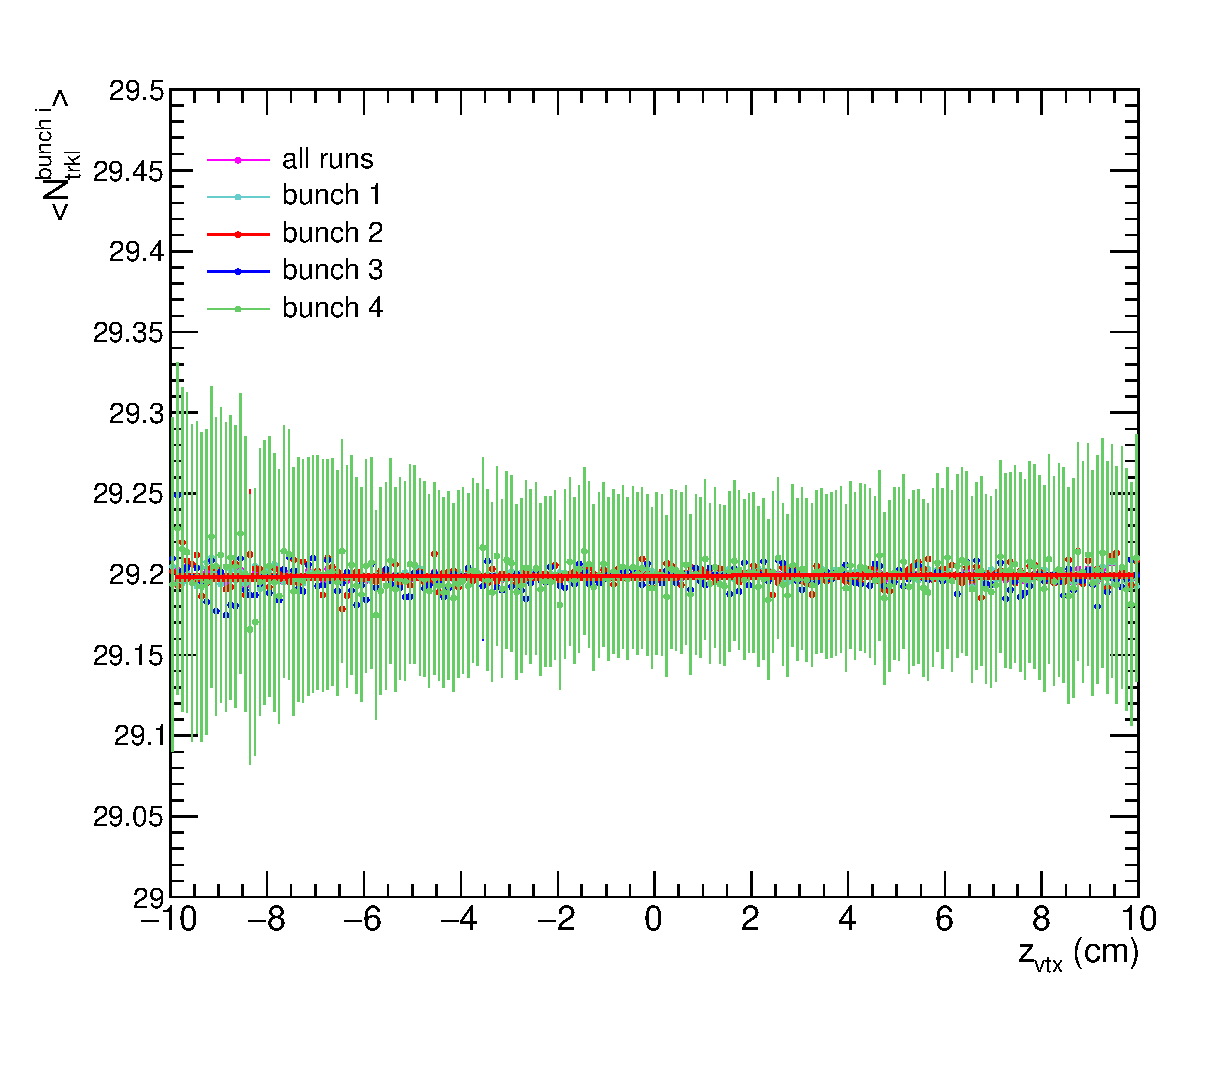
\includegraphics[width=.465\textwidth]{FigCap6/NtrkProfilesDataAfterZVxtEqual.eps}
 \caption{Left: average $\Ntrkl$ distributions as a function of the z-vertex coordinate for the four bunches of runs in different colours. Right: average $\Ntrkl$ distributions as a function of the z-vertex coordinate for the four bunches of runs in different colours after the equalisation on the z-vertex coordinate.}
 \label{fig:FourBunches}
\end{figure}

\subsection {Raw-yield extraction}
\label{sec:Rawyields_vs_mult}
The $\Ds$ and $\Dplus$ mesons were reconstructed in the central rapidity region together with their anti-particle from the hadronic decay channels
$\DstophipitoKKpi$  with a branching ratio, BR, of $2.27 \pm0.08\%$ and $\DplustoKpipi$ with BR of $9.46\pm0.24 \%$), as was done for the analyses described in the previous sections (see Sec.~\ref{sec:Reconstruction}). For this analysis, the $\Ds$ and $\Dplus$ signal was extracted in 5 $\pt$ intervals for 3 different classes of $N_{\rm trkl}$:
\begin{itemize}
\item $1 \leq N_{\rm trkl} < 40$
\item $40 \leq N_{\rm trkl} < 70$
\item $70 \leq N_{\rm trkl} \leq 200$
\end{itemize}
For the $\Dplus$, the same topological selection used for the $R_{\rm pPb}$ and $\QpPb/\Qcp$ analyses were applied, while for the $\Ds$ the selections were optimized to have a good signal extraction in each $\pt$ and $N_{\rm trkl}$ interval. The $\Ds$ topological selections applied in all the $N_{\rm trkl}$ classes of events are summarized in table \ref{tab:cutsDsVsNtrkl}. The same single-track selections of the analyses described above were applied.

\begin{table}[h!]
\centering
\begin{tabular}{|l|c|c|c|c|c|}
\hline
$\Ds$ topological selections & \multicolumn{5}{c|}{pt interval (GeV/$c$)}\\
\cline{2-6}
  & 2--4  & 4--6 & 6--8 & 8--12 & 12--16\\
\hline
Decay length ($\mum$)        & $>$300 & $>$350 & $>$350 & $>$400& $>$400\\
Decay length XY ($\mum$)     & $>$0 & $>$200 & $>$200 & $>$200 & $>$200\\
Norm Decay length XY          & $>$2.0& $>$0.0 & $>$2.0 & $>$2.0 & $>$2.0\\
Cosine pointing              & $>$0.94 & $>$0.95 & $>$0.95 & $>$0.97 & $>$0.97\\
$\sigma_{vertex}$  (cm)          & $<$0.02 & $<$0.03 & $<$0.03 & $<$0.06 & $<$0.06\\
M$^{\phi}_{inv}$ - M$^{\phi PDG}_{inv}$ (MeV/$c^{2}$) & $<$8.0 & $<$10.0 & $<$4.5 & $<$9.0 & $<$9.0\\
$\cos \theta^*(\pi)$    & $<$1.0 & $<$1.0 & $<$1.0 & $<$0.95 & $<$0.95\\
$|\cos^3 \theta^\prime({\rm K})|$        & $>$0.10 & $>$0.05 & $>$0.05 & $>$0.05 & $>$0.05\\
Norm. IP residual  & $<$2.5 & $<$2.0 & $<$2.0 & $<$2.0  & $<$2.0 \\
\hline
\end{tabular}
\caption{Topological selections used for the $\Ds$ meson in the five transverse momentum intervals consideredfor the three $N_{\rm trkl}$ classes.}
\label{tab:cutsDsVsNtrkl}
\end{table}

Figures~\ref{fig:DplusInvMassVsNtrkl_1},~\ref{fig:DplusInvMassVsNtrkl_2},~\ref{fig:DplusInvMassVsNtrkl_3}  and~\ref{fig:DsInvMassVsNtrkl_1},~\ref{fig:DsInvMassVsNtrkl_2},~\ref{fig:DsInvMassVsNtrkl_3} show the invariant-mass fits performed to extract the signal in each $\pt$ interval for the three classes of $N_{\rm trkl}$, for $\Dplus$ and $\Ds$ respectively. 

\begin{figure}[htpb]
\centering
 \includegraphics[width=.9\textwidth]{FigCap6/RawYields_Central_d0Cut_Ntrklts_1_39_sigmafixtoMB.pdf}
 \caption{$\Dplus$ invariant-mass spectra in 5 $\pt$ intervals from 2 to 16 $\Gevc$ for the $1 \leq N_{\rm trkl} < 40$ interval.}
 \label{fig:DplusInvMassVsNtrkl_1}
\end{figure}

\begin{figure}[htpb]
\centering
 \includegraphics[width=.9\textwidth]{FigCap6/RawYields_Central_d0Cut_Ntrklts_40_69_sigmafixtoMB.pdf}
 \caption{$\Dplus$ invariant-mass spectra in 5 $\pt$ intervals from 2 to 16 $\Gevc$ for the $40 \leq N_{\rm trkl} < 70$ interval.}
 \label{fig:DplusInvMassVsNtrkl_2}
\end{figure}

\begin{figure}[htpb]
\centering
 \includegraphics[width=.9\textwidth]{FigCap6/RawYields_Central_d0Cut_Ntrklts_70_200_sigmafixtoMB.pdf}
 \caption{$\Dplus$ invariant-mass spectra in 5 $\pt$ intervals from 2 to 16 $\Gevc$ for the $70 \leq N_{\rm trkl} \leq 200$ interval.}
 \label{fig:DplusInvMassVsNtrkl_3}
\end{figure}

\begin{figure}[htpb]
\centering
 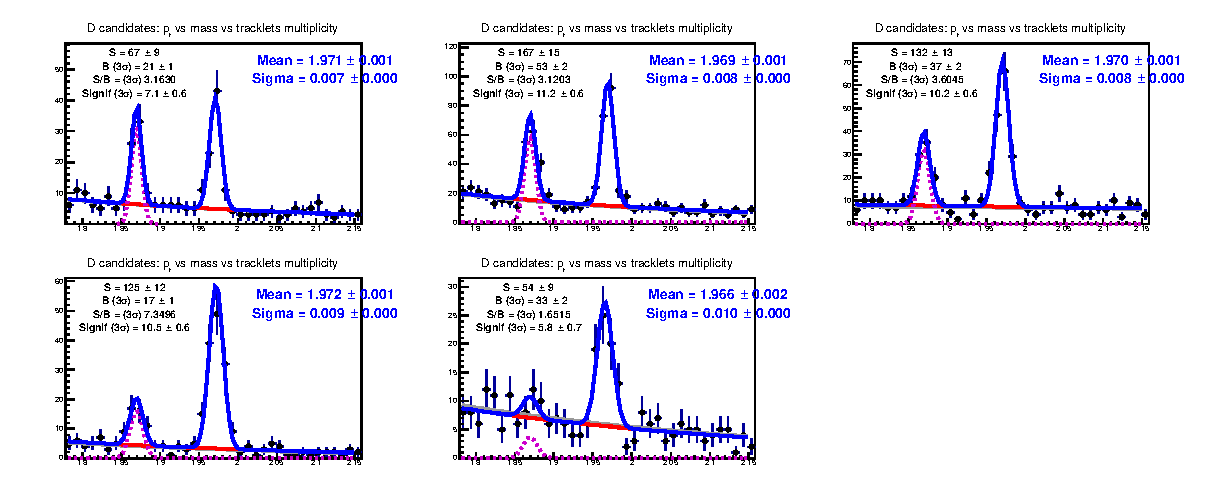
\includegraphics[width=.9\textwidth]{FigCap6/DsMass140.eps}
  \caption{$\Ds$ invariant-mass spectra in 5 $\pt$ intervals from 2 to 16 $\Gevc$ for the $1 \leq N_{\rm trkl} < 40$ interval.}
 \label{fig:DsInvMassVsNtrkl_1}
\end{figure}

\begin{figure}[htpb]
\centering
 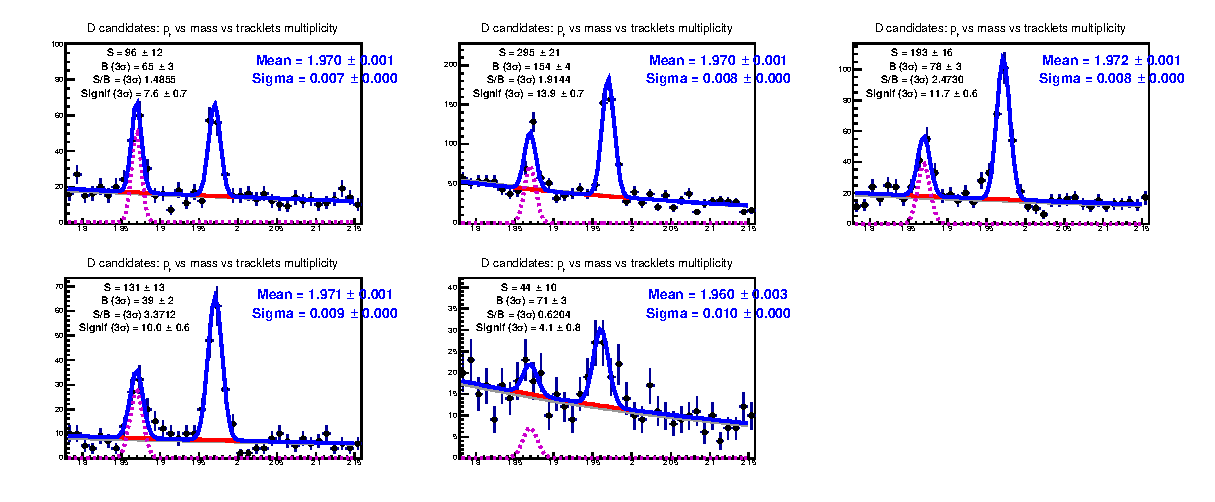
\includegraphics[width=.9\textwidth]{FigCap6/DsMass4070.eps}
 \caption{$\Ds$ invariant-mass spectra in 5 $\pt$ intervals from 2 to 16 $\Gevc$ for the $40 \leq N_{\rm trkl} < 70$ interval.}
 \label{fig:DsInvMassVsNtrkl_2}
\end{figure}

\begin{figure}[htpb]
\centering
 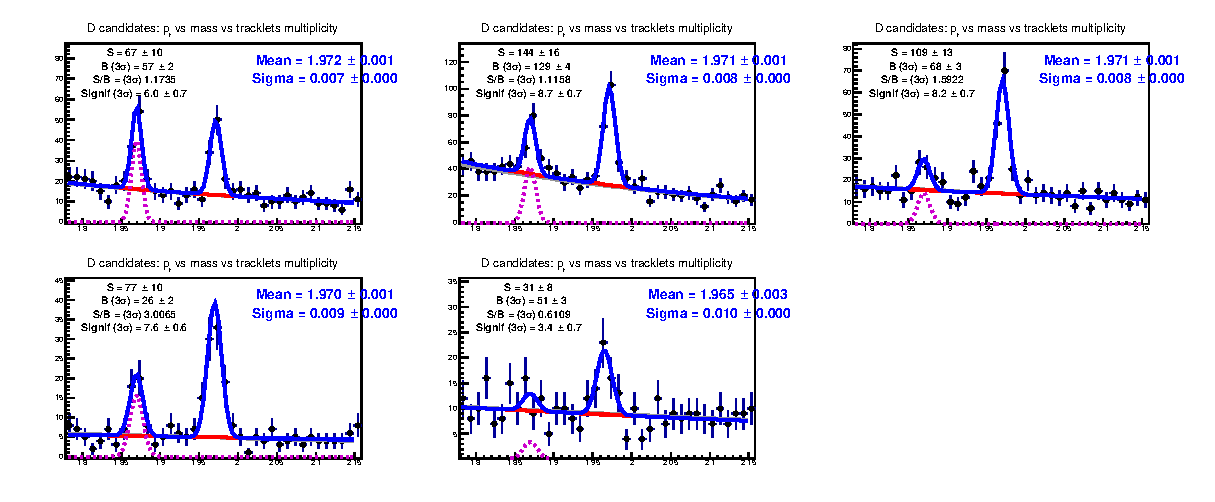
\includegraphics[width=.9\textwidth]{FigCap6/DsMass70200.eps}
 \caption{$\Ds$ invariant-mass spectra in 5 $\pt$ intervals from 2 to 16 $\Gevc$ for the $70 \leq N_{\rm trkl} \leq 200$ interval.}
 \label{fig:DsInvMassVsNtrkl_3}
\end{figure}

For the $\Dplus$ the peak width was fixed to the one obtained from the fit to the minimum bias sample in the same $\pt$ interval to reduce statistical fluctuation, since the mass resolution does not show a dependence on the multiplicity, as shown in Fig.~\ref{fig:DplusFitParamsVsNtrkl}. For the same reason the $\Ds$ peak was fixed to the value obtained from the MC simulation, which was verified to be compatible to the one of data in the minimum bias sample. In Fig.~\ref{fig:DsFitParamsVsNtrkl} the comparison of the $\Ds$ (and $\Dplus$ in the same $\Ds$ decay channel) peak for  data in the interval $40 \leq N_{\rm trkl} < 70$ and the minimum-bias MC simulation is shown. 

\begin{figure}[htpb]
\centering
 \includegraphics[width=.45\textwidth]{FigCap6/Sigma_Ntrklts_1_40_70_200_Pt_2_4_6_8_12_16.pdf}
 \includegraphics[width=.45\textwidth]{FigCap6/Mean_Ntrklts_1_40_70_200_Pt_2_4_6_8_12_16.pdf}
  \caption{$\Dplus$ peak width (left) and mean (right) obtained in the $N_{\rm trkl}$ intervals compared to the values from the minimum-bias data sample and the MC simulation.}
 \label{fig:DplusFitParamsVsNtrkl}
\end{figure}

\begin{figure}[htpb]
\centering
 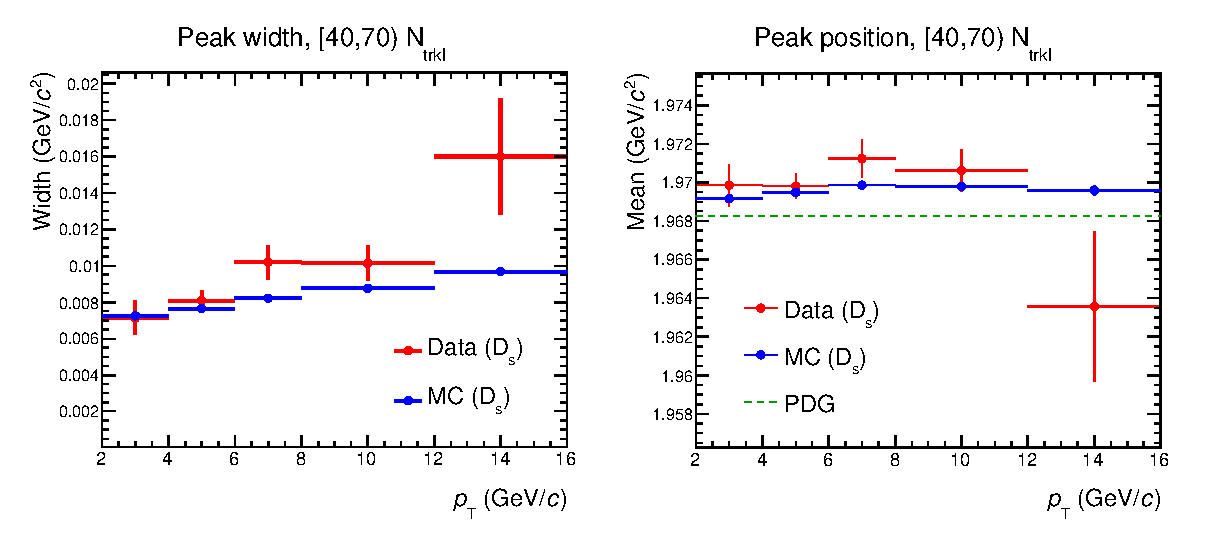
\includegraphics[width=.9\textwidth]{FigCap6/DsMeanSigma_DataMC_4070_Ntrkl.eps}
  \caption{$\Ds$ (and $\Dplus$ in the same $\Ds$ decay channel) peak width (left) and mean (right) obtained in the $N_{\rm trkl}$ intervals compared to the values from the data in the interval $40 \leq N_{\rm trkl} < 70$ and the minimum-bias MC simulation.}
 \label{fig:DsFitParamsVsNtrkl}
\end{figure}

\subsection {$N_{\rm tracklets}$ weights}
\label{fig:NtrklWeights_vsMult}

A further correction is needed for the Monte Carlo efficiencies, after the z-vertex equalisation already made on data,
since the tracklet distributions in data and in MC are indeed different, as can be seen in Fig.~\ref{fig:NtrklDataMC}.
The numerator and denominator of the MC efficiencies were hence multiplied by a correction factor, 
defined as the ratio of the $\Ntrkl$ in data and in MC for a given event tracklet multiplicity.
From the $\Ntrkl$ distributions of Fig.~\ref{fig:NtrklDataMC} it can be seen that the simulated distribution reaches
lower values of $\Ntrkl$ with respect to data, but it was checked that the D-meson efficiencies does not depend on
the tracklet multiplicity above the 20 tracklets per event.
The correction factor was calculated independently for each of the four bunches of runs described in Sec.~\ref{subsec:zVxtEq} (Fig.~\ref{Weights4Bunches}),
since also the inclusive distribution of the tracklets showed differences versus time related to the variation of the SPD configuration during the
period of data taking. In Fig.~\ref{NtrklWeights4BunchesRatioToMB} the ratio of the tracklet distributions for each of the four bunches
of runs to that obtained considering the full runlist is shown, to better clarify the necessity of four distinct corrections.


\begin{figure}[h]
\centering
 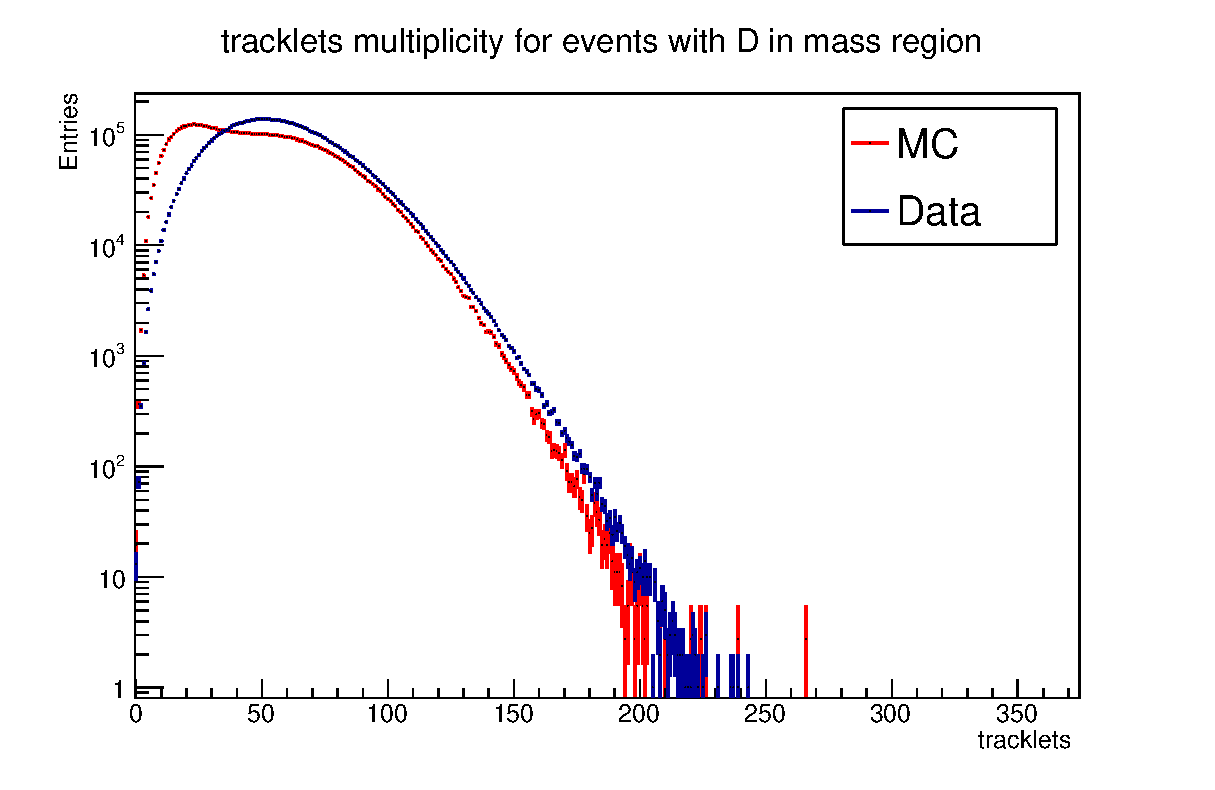
\includegraphics[width=.49\textwidth]{FigCap6/NtrkDistrWithDDataMC.eps}
 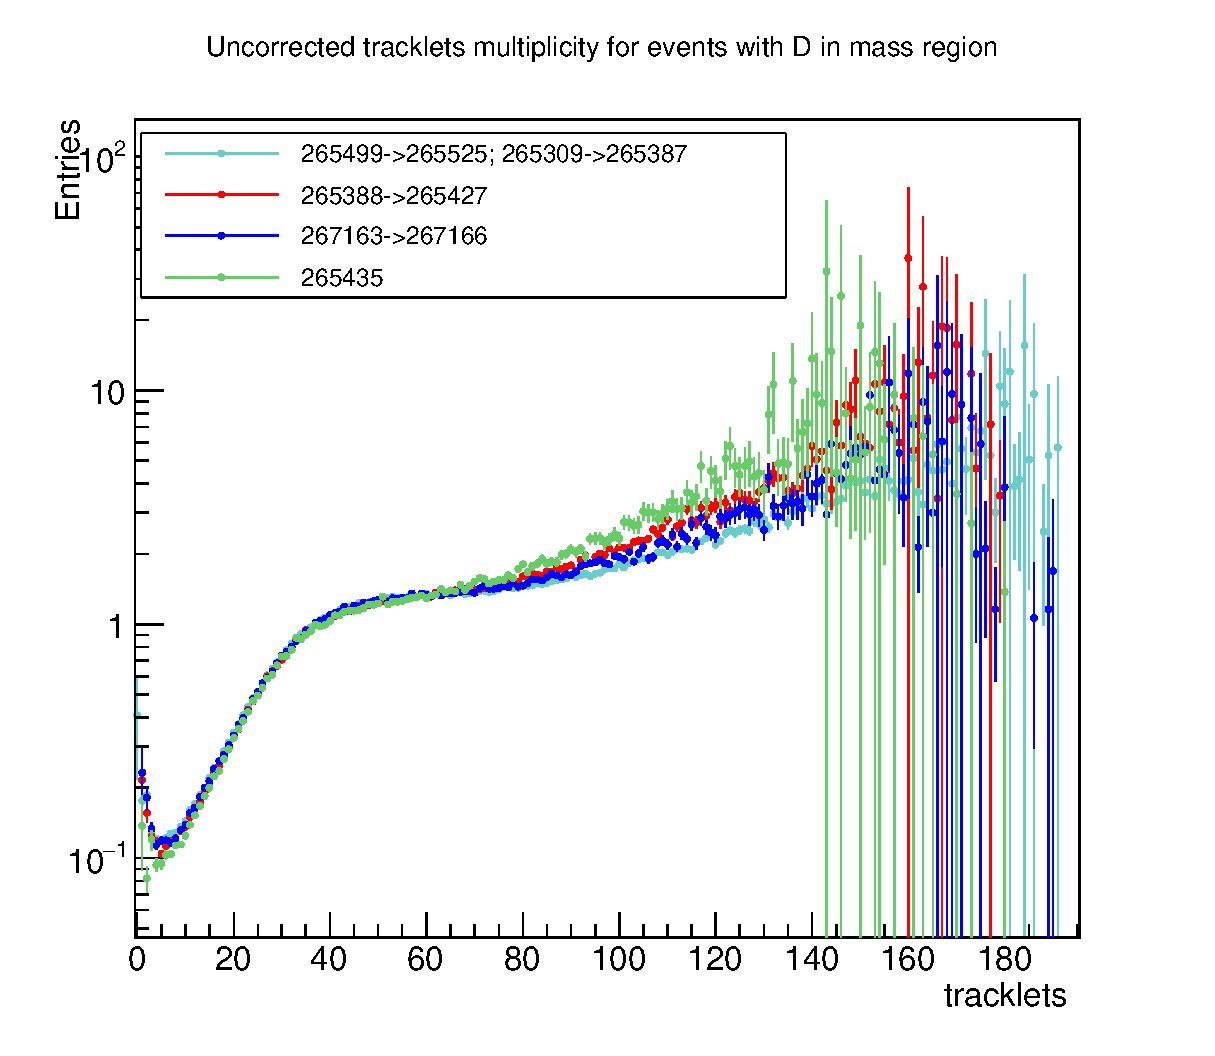
\includegraphics[width=.43\textwidth]{FigCap6/NtrklWeights4Bunches.eps}
 \caption{Left: tracklets distribution in data and in MC in different colours. Right: $\Ntrkl$-weight distributions for the MC in each of the four bunches of runs in different colours.}
 \label{fig:NtrklDataMC}
\end{figure}

\begin{figure}[h]
\centering
 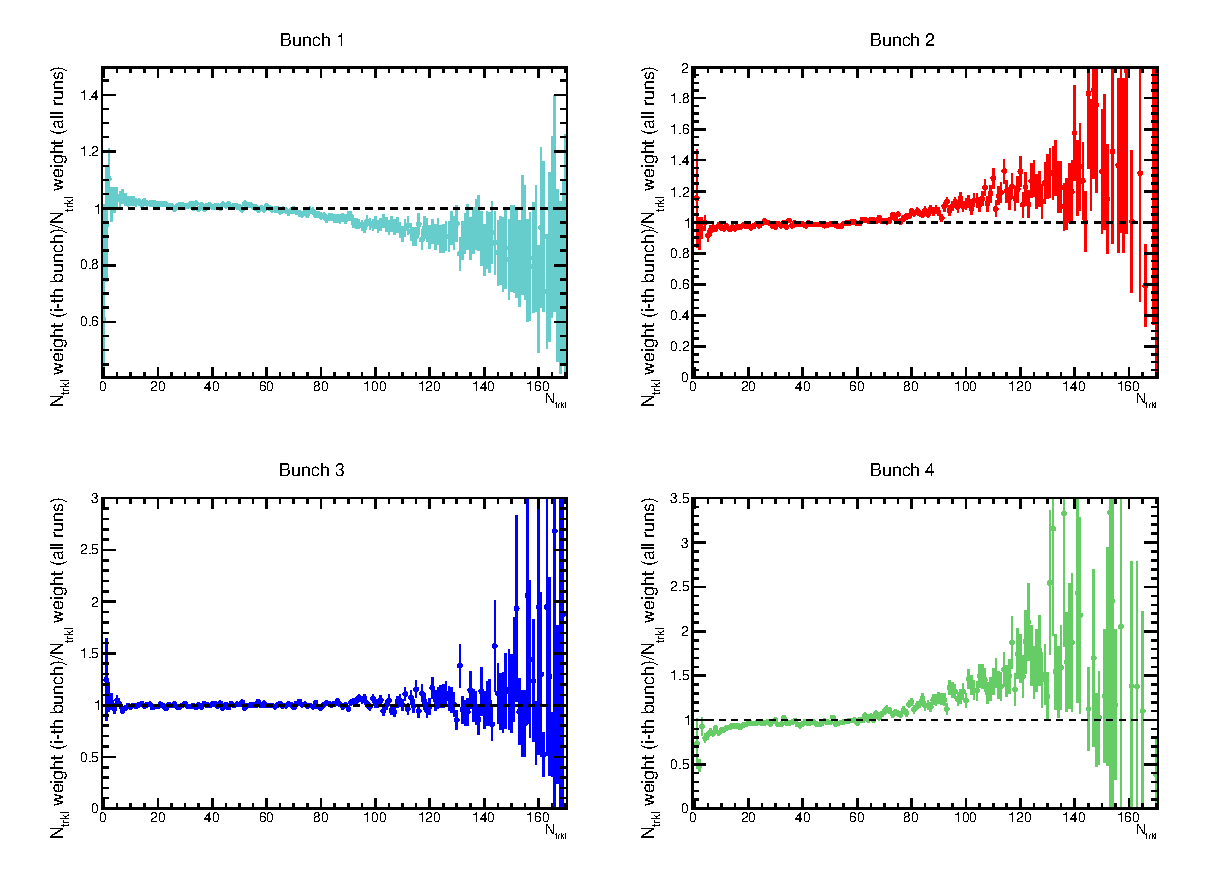
\includegraphics[width=.85\textwidth]{FigCap6/NtrkDistrMC_17d2a_EvWithD_zVxtUnCorr_896_897.eps}
 \caption{Ratio of the $\Ntrkl$ distribution for the MC in each of the four bunches of runs over the distribution obtained with the full statistics.}
 \label{fig:NtrklDataMC}
\end{figure}

\begin{figure}[h]
\centering
 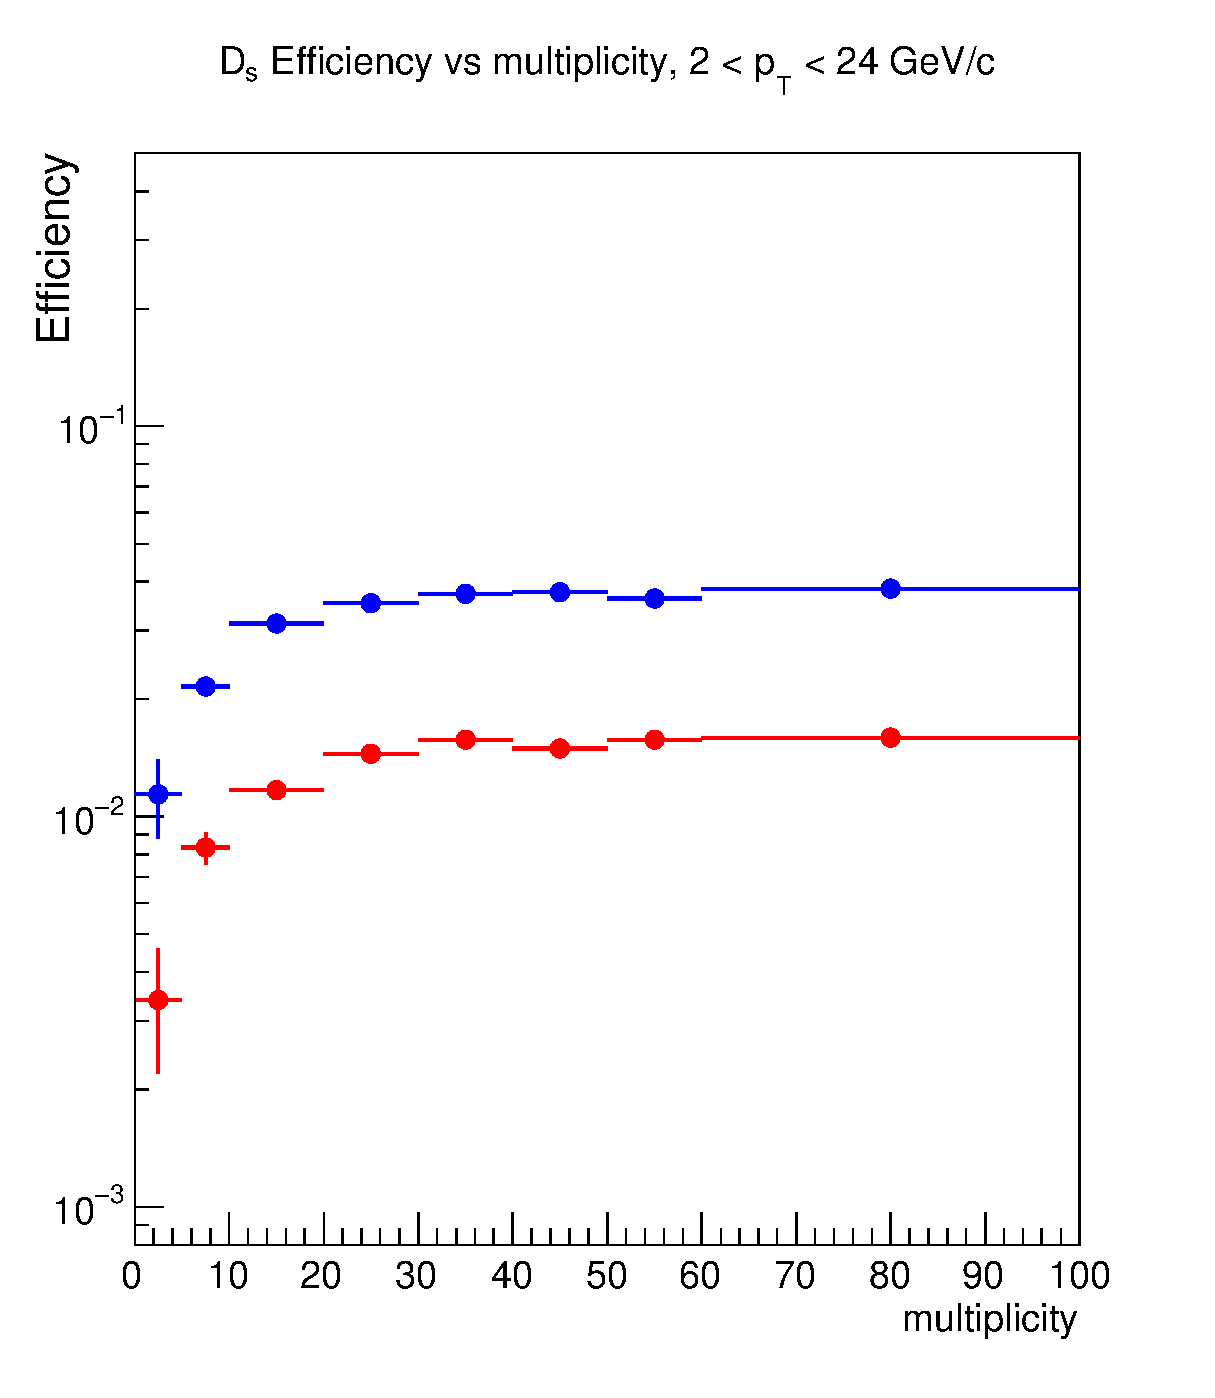
\includegraphics[width=.45\textwidth]{FigCap6/DsEffvsMult_pPb2016.eps}
 \caption{$\Ds$ efficiency as a function of the tracklet multiplicity, $\pt$-integrated between 2 and 24 $\Gevc$, in red for prompt and in blue for the feed-down.}
 \label{fig:DsEffVsMult}
\end{figure}

\subsection {Efficiencies and acceptance}
The efficiency and acceptance factors for the $\Ds$ and the $\Dplus$, were computed as described in Sec.~\ref{subsec:eff}. For the multiplicity weights, four different distributions, corresponding to the four bunches of runs with the different $Z_{\rm vtx}$ correction were used, as explained in the previous section. The resulting efficieny times acceptance factors are shown in Fig.~\ref{fig:DplusEffAccVsNtrkl} for the $\Dplus$ as a function of $N_{\rm trkl}$ and for the $\Ds$ as a function of $\pt$ are shown in Fig.~\ref{DplusEffAccVsNtrkl} and Fig.~\ref{DsEffAccVsNtrkl} respectively. As shown in these figures, the efficiency is almost flat as a function of the event multiplicity, and the largest difference is observed between the first $N_{\rm trkl}$ interval and the other two, as expected.

\begin{figure}[htpb]
\centering
 \includegraphics[width=.45\textwidth]{FigCap6/Efficiency_times_Acceptance_VsNtrkl_Central_d0Cut_ImpTask_Prompt.pdf}
 \includegraphics[width=.45\textwidth]{FigCap6/Efficiency_times_Acceptance_VsNtrkl_Central_d0Cut_ImpTask_FD.pdf}
  \caption{Prompt (left) and feed-down (right) $\Dplus$ efficiency times acceptance factor as a function of $N_{\rm trkl}$ for the $\pt$ intervals considered in the analysis.}
 \label{fig:DplusEffAccVsNtrkl}
\end{figure}


\subsection {Feed-down subtraction}
For the feed-down subtraction the FONLL-based $N_{\rm b}$ method was used (see Sec~\ref{sec:FeedDown_Nb}). In particular, it was assumed that the fraction of prompt D does not depend on the multiplicity and therefore $f_{\rm prompt}$ was computed considering the minimum bias sample for all the $N_{\rm trkl}$ classes. This hypothesis is also supported by the result obtained for the $\QpPb$ analysis, for which it was found that the fraction of prompt D is very similar in the two ZNA centrality classes and in the minimum bias sample (see Fig.~\ref{fig:DplusPromptFrac_010_60100}). In particular, it was assumed that $R_{\rm pPb}^{\rm feed-down} = R_{\rm pPb}^{\rm prompt}$ for both $\Ds$ and $\Dplus$, as done for the minimum bias analysis. This hypothesis has been then varied between $0.9 < R_{\rm pPb}^{\rm feed-down} = R_{\rm pPb}^{\rm prompt} <1.3$ to estimate a systematic uncertainty, as will be described in more details in the dedicated section. In Fig~\ref{fig:DplusfPromptVsNtrkl} the fraction of prompt $\Dplus$ in the $\pt$ intervals of the analysis is shown.

\begin{figure}[htpb]
\centering
 \includegraphics[width=.7\textwidth]{FigCap6/DplusFprompt_Nb_d0cut_1_200.pdf}
  \caption{Fraction of prompt $\Dplus$ in the $\pt$ intervals considered for the analysis.}
 \label{fig:DplusfPromptVsNtrkl}
\end{figure}

\subsection {Systematic uncertainties}
\subsubsection{Raw-yield extraction}
The systematic uncertainty due to the raw-yield extraction was estimated using the same strategy adopted for the analyses described above (see Sec.~\ref{sec:rawyieldsyst}). This approach is based on repeating many times the invariant-mass fit, combining in all the possible ways different fit configurations. In particular, the following quantities have been varied:
\begin{itemize}
\item fit range
\item invarian-mass binning
\item background fit function (exponential, linear and parabolic)
\item peak width free and fixed to the value obtained from the minimum-bias sample ($\Dplus$) and MC simulation ($\Ds$)
\item peak mean free and fixed to the PDG value
\end{itemize} 
Moreover, the result was compared to the values obtained with a bin counting method, and a good fit quality was required, applying a selection on the chi square ($\chi^2<3$). Figures~\ref{fig:DplusMultiTrial_1},~\ref{fig:DplusMultiTrial_2},~\ref{fig:DplusMultiTrial_3} and ~\ref{fig:DsMultiTrial_1},~\ref{fig:DsMultiTrial_2},~\ref{fig:DsMultiTrial_3} show an example of multi-trial output for each $\Ntrkl$ interval considered in the anlysis, for $\Dplus$ and $\Ds$ respectively.  
 
 \begin{figure}[htpb]
\centering
 \includegraphics[width=.9\textwidth]{FigCap6/RawYieldsSyst_Central_d0cut_Ntrklts_1_39_pt3.pdf}
 \caption{Output of multi-trial fits to $\Dplus$ invariant mass distributions for the $1 \leq \Ntrkl < 40$ class in the $\pt$ interval $ 8 < \pt < 12$ $\GeV/c$.}
 \label{fig:DplusMultiTrial_1}
\end{figure}

 \begin{figure}[htpb]
\centering
 \includegraphics[width=.9\textwidth]{FigCap6/RawYieldsSyst_Central_d0cut_Ntrklts_40_69_pt2.pdf}
 \caption{Output of multi-trial fits to $\Dplus$ invariant mass distributions for the $40 \leq \Ntrkl < 70$ class in the $\pt$ interval $ 6 < \pt < 8$ $\GeV/c$.}
 \label{fig:DplusMultiTrial_2}
\end{figure}

\begin{figure}[htpb]
\centering
 \includegraphics[width=.9\textwidth]{FigCap6/RawYieldsSyst_Central_d0cut_Ntrklts_70_200_pt0.pdf}
 \caption{Output of multi-trial fits to $\Dplus$ invariant mass distributions for the $70 \leq \Ntrkl \leq 200$ class in the $\pt$ interval $ 2 < \pt < 4$ $\GeV/c$.}
 \label{fig:DplusMultiTrial_3}
\end{figure}

 \begin{figure}[htpb]
\centering
 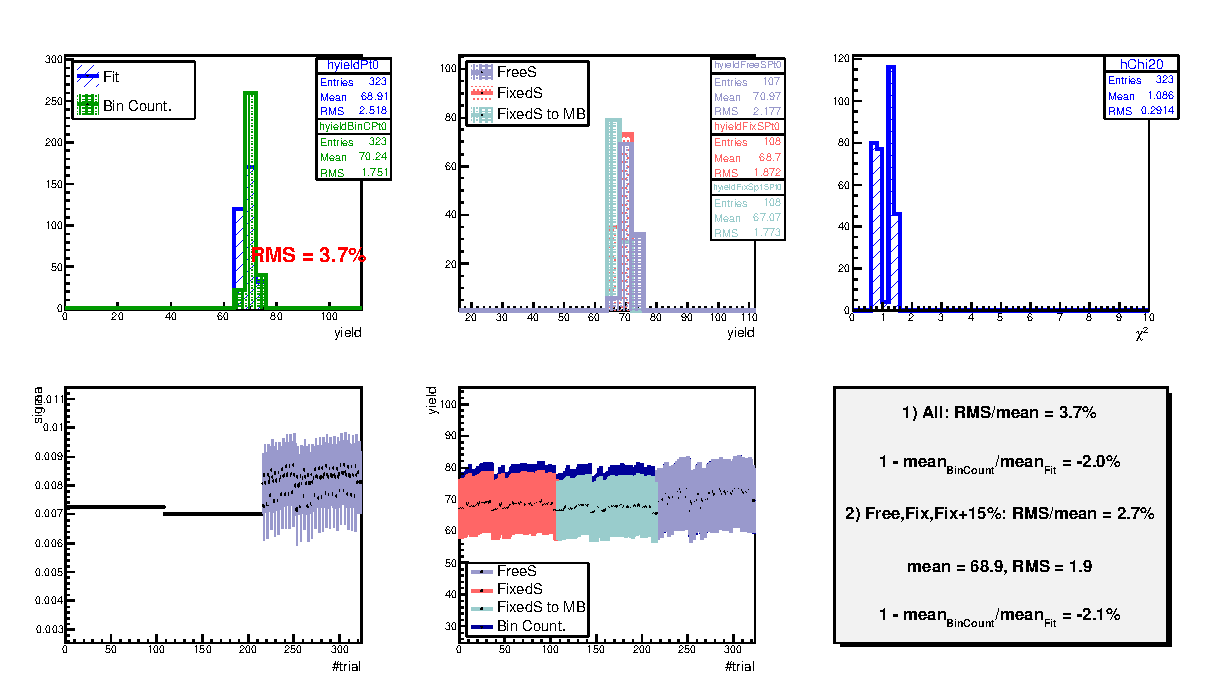
\includegraphics[width=.9\textwidth]{FigCap6/MT_Pt0_140.eps}
 \caption{Output of multi-trial fits to $\Ds$ invariant mass distributions for the $1 \leq \Ntrkl < 40$ class in the $\pt$ interval $ 2 < \pt < 4$ $\GeV/c$.}
 \label{fig:DplusMultiTrial_1}
\end{figure}

 \begin{figure}[htpb]
\centering
 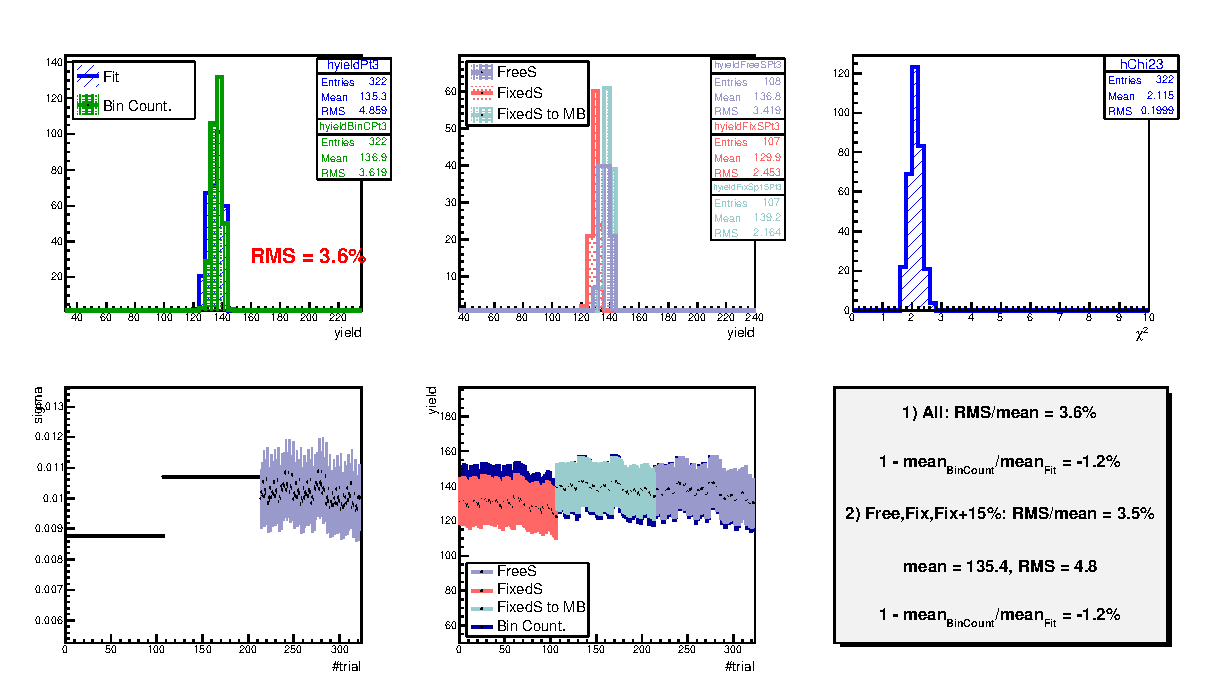
\includegraphics[width=.9\textwidth]{FigCap6/MT_Pt3_4070.eps}
 \caption{Output of multi-trial fits to $\Ds$ invariant mass distributions for the $40 \leq \Ntrkl < 70$ class in the $\pt$ interval $  8< \pt < 12$ $\GeV/c$.}
 \label{fig:DplusMultiTrial_2}
\end{figure}

\begin{figure}[htpb]
\centering
 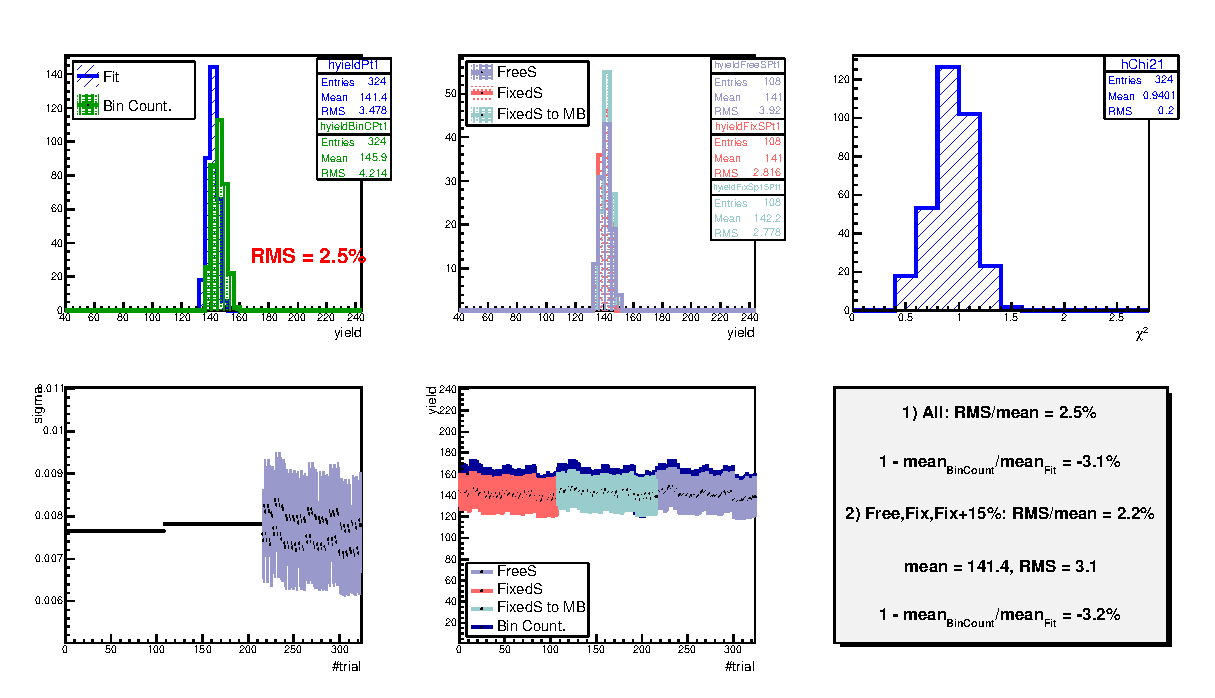
\includegraphics[width=.9\textwidth]{FigCap6/MT_Pt1_70200.eps}
 \caption{Output of multi-trial fits to $\Ds$ invariant mass distributions for the $70 \leq \Ntrkl \leq 200$ class in the $\pt$ interval $  4< \pt < 6$ $\GeV/c$.}
 \label{fig:DplusMultiTrial_3}
\end{figure}

The values assigned as systematic uncertainties are summarized in Tab.~\ref{tab:DplusVsMult_syst} and~\ref{tab:DsVsMult_syst} for $\Dplus$ and $\Ds$ respectively.

\subsubsection{MC $N_{\rm tracklets}$ distribution}
Since the MC simulation does not reproduce the multiplicity of the data, the D-meson efficiencies were reweighted according to the $N_{\rm tracklets}$ distribution measured in the data, as described in section~\ref{sec:NtrklWeights_vsMult}. In order to check the stability of the efficiencies and to estimate a possible systematic uncertainty, the $\Dplus$ and $\Ds$ efficiencies were reweighted considering the distribution of $\Ntrkl$ obtained from the events that have at least a $\Dzero$ meson candidate, without requiring that the invariant mass of the candidates is compatible to the one of the $\Dzero$. In Fig.~\ref{fig:NtrklWeights_EvWithD_EvWithCand_Comparison} the comparison between the weights used as default and those used to estimate a systematic uncertainty is shown for the four different bunches of runs (see Sec.~\ref{subsec:zVxtEq}).

\begin{figure}[htpb]
\centering
 \includegraphics[width=.9\textwidth]{FigCap6/NtrkWeightsD-Cand_4Bunches_DsDplusVsmult.pdf}
 \caption{Comparison of the $\Ntrkl$ weights obtained from events with at least a $\Dzero$ candidate to those obtained from events with at least a $\Dzero$ candidate in the $\Dzero$ mass range (default).}
 \label{fig:NtrklWeights_EvWithD_EvWithCand_Comparison}
\end{figure}

Fig.~\ref{fig:DsDplusVsMult_SystEffWeights} shows the ratio between the efficiency obtained with these weights, compared to the default ones, for $\Dplus$ (right) and $\Ds$ (left). Since the variation is smaller than 1\% for the $\Dplus$ the effect was considered as negligible, wile for the $\Ds$ a 1\% was assigned.

\begin{figure}[htpb]
\centering
 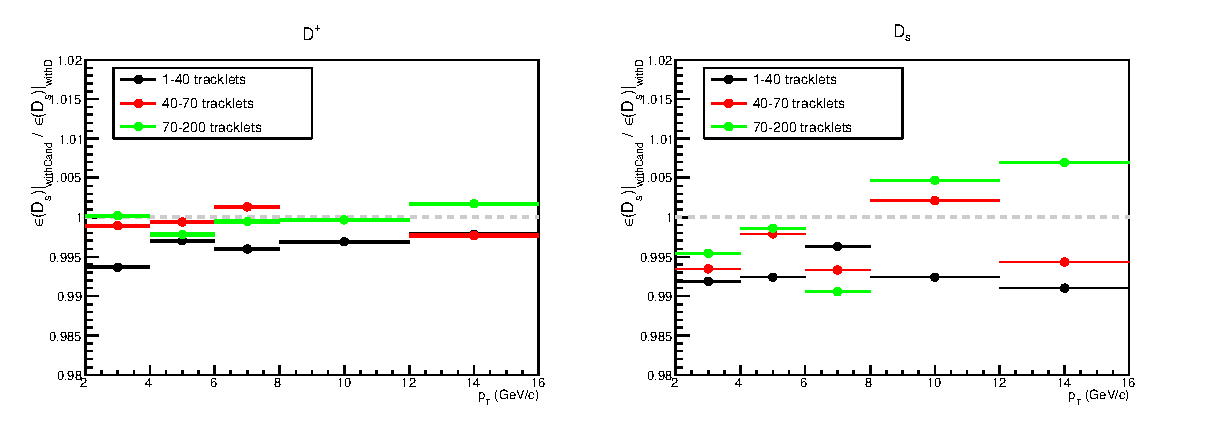
\includegraphics[width=.9\textwidth]{FigCap6/SystOnDWeightsWithCandVsWithD.eps}
 \caption{Ratio between the efficiency obtained with these weights, compared to the default ones, for $\Dplus$ (right) and $\Ds$ (left).}
 \label{fig:DsDplusVsMult_SystEffWeights}
\end{figure}

\subsubsection{Feed-down subtraction}
The feed-down subtraction has been performed using the $N_{\rm b}$ method considering the full minimum-bias sample, assuming that the fraction of prompt D mesons was the same in the different $\Ntrkl$ classes of events. Also the systematic uncertainty on the prompt fraction is the same as the one evaluated for the minimum-bias sample. It comes from (i) the variation of the FONLL parameters (mainly from the renormalization scale) and (ii) the hypothesis on the $\RpPb$ of feed-down D mesons. In particular this hypothesis was varied in the range $0.9 <\RpPb^{\rm feed-down}/\RpPb^{\rm prompt} < 1.3$.

\subsubsection{Topological selection efficiency}
Since the D meson efficiency depends only slightly on the multiplicity (e.g. see Fig.~\ref{fig:DplusEffAccVsNtrkl}) and the same topological selections were applied in the different $\Ntrkl$ intervals, the systematic uncertainty was considered to be the same as the one estimated for the minimum-bias analysis.

\subsubsection{PID efficiency}
The PID efficiency is not expected to vary significantly with the multiplicity, and therefore the uncertainty on the PID selection efficiency was considered to be the same as the one estimated for the minimum-bias analysis. This is also supported by the study performed for the $\Dplus$ in the two ZNA classes of events considered for the $\QpPb$ analysis (see Sec.\ref{sec:PIDsyst}).

\subsubsection{MC $\pt$ shape}
As for the minimum-bias analysis also for the $\Ds/\Dplus$ as a function of multiplicity, the systematic uncertainty due to the MC $\pt$ shape was considered as negligible.

\subsubsection{Tracking efficiency}
The tracking efficiency is not expected to vary significantly with the multiplicity, and therefore the uncertainty on the tracking efficiency was considered to be the same as the one estimated for the minimum-bias analysis.

\subsubsection{Total systematic uncertainties}
In Tables~\ref{tab:DplusVsMult_syst} and~\ref{tab:DsVsMult_syst} the values of the systematic uncertainties for the $\Dplus$ and the $\Ds$ are summarized.
In the $\Ds/\Dplus$ ratio the following sources of systematic uncertainties were considered as uncorrelated:
\begin{itemize}
\item Raw-yield extraction
\item Topological selection efficiency
\item PID selection efficieny
\item MC $\pt$ shape (negligible)
\item Hypothesis on $\RpPb^{feed-down}$ for the feed-down D meson subtraction
\end{itemize} 
while
\begin{itemize}
\item MC $\Ntrkl$ distribution
\item Tracking efficiency
\item FONLL scale for the feed-down D meson subtraction
\end{itemize} 
as fully correlated.

\begin{table}[h!]
\centering
\scalebox{0.9}{
\begin{tabular}{|l|c|c|c|c|c|}
\hline
 $\Dplus$ syst. unc. (\%) & \multicolumn{5}{c|}{$\pt$ interval ($\GeV/c$)}\\
\hline
 $1 \leq \Ntrkl < 40$ & 2--4  & 4--6 & 6--8 & 8--12 & 12--16 \\
\hline
Feed-down above &1.5  & 2 & 2	& 2.5 & 2.5\\
Feed-down below & 2 & 3 & 3	& 4 & 4 \\
Cut variation & 5.5 & 4 & 4 & 4 & 4\\
Raw yield  & 2 & 2 & 2 & 2 & 4\\
MC $\pt$-shape & negl & negl & negl & negl & negl \\
PID &  negl & negl & negl & negl & negl \\
Tracking & 4 & 4 & 4 & 4 & 4 \\
Multiplicity weights & negl &  negl &  negl &  negl &  negl \\
\hline
 $40 \leq \Ntrkl < 70$ & 2--4  & 4--6 & 6--8 & 8--12 & 12--16 \\
\hline
Feed-down above &1.5  & 2 & 2	& 2.5 & 2.5\\
Feed-down below & 2 & 3 & 3	& 4 & 4 \\
Cut variation & 5.5 & 4 & 4 & 4 & 4\\
Raw yield  & 2 & 2 & 2 & 2 & 4\\
MC $\pt$-shape & negl & negl & negl & negl & negl \\
PID &  negl & negl & negl & negl & negl \\
Tracking & 4 & 4 & 4 & 4 & 4 \\
Multiplicity weights & negl &  negl &  negl &  negl &  negl \\
\hline
 $70 \leq \Ntrkl < 200$ & 2--4  & 4--6 & 6--8 & 8--12 & 12--16 \\
\hline
Feed-down above &1.5  & 2 & 2	& 2.5 & 2.5\\
Feed-down below & 2 & 3 & 3	& 4 & 4 \\
Cut variation & 5.5 & 4 & 4 & 4 & 4\\
Raw yield  & 3 & 2 & 2 & 3 & 4\\
MC $\pt$-shape & negl & negl & negl & negl & negl \\
PID &  negl & negl & negl & negl & negl \\
Tracking & 4 & 4 & 4 & 4 & 4 \\
Multiplicity weights & negl &  negl &  negl &  negl &  negl \\
\hline
\end{tabular}}
\caption{Systematic uncertainties on $\Dplus$ for the $\Ds/\Dplus$ vs. multiplicity measurement.}
\label{tab:DplusVsMult_syst}
\end{table}

\begin{table}[h!]
\centering
\scalebox{0.9}{
\begin{tabular}{|l|c|c|c|c|c|}
\hline
 $\Ds$ syst. unc. (\%) & \multicolumn{5}{c|}{$\pt$ interval ($\GeV/c$)}\\
\hline
 $1 \leq \Ntrkl < 40$ & 2--4  & 4--6 & 6--8 & 8--12 & 12--16 \\
\hline
Feed-down above &	3	& 3 &3 & 3	&5\\
Feed-down below &	4	&4 &4 &4 &5 \\
Cut variation & 14 & 9 & 8	& 8	&7\\
Raw yield  & 4 & 4 & 3 & 3 & 9\\
MC $\pt$-shape & negl & negl & negl & negl & negl \\
PID &  2 & 2 & 2 & 2 & 2 \\
Tracking & 4 & 4 & 4 & 4 & 4 \\
Multiplicity weights & 1 &  1 &  1 &  1 &  1 \\
\hline
 $40 \leq \Ntrkl < 70$ & 2--4  & 4--6 & 6--8 & 8--12 & 12--16 \\
\hline
Feed-down above &	3	& 3 &3 & 3	&5\\
Feed-down below &	4	&4 &4 &4 &5 \\
Cut variation & 14 & 9 & 8	& 8	&7\\
Raw yield  & 3 & 3 & 4 & 5 & 12\\
MC $\pt$-shape & negl & negl & negl & negl & negl \\
PID &  2 & 2 & 2 & 2 & 2 \\
Tracking & 4 & 4 & 4 & 4 & 4 \\
Multiplicity weights & 1 &  1 &  1 &  1 &  1 \\
\hline
 $70 \leq \Ntrkl < 200$ & 2--3  & 4--6 & 6--8 & 8--12 & 12--16 \\
\hline
Feed-down above &	3	& 3 &3 & 3	&5\\
Feed-down below &	4	&4 &4 &4 &5 \\
Cut variation & 14 & 9 & 8	& 8	&7\\
Raw yield  & 4 & 4 & 4 & 4 & 10\\
MC $\pt$-shape & negl & negl & negl & negl & negl \\
PID &  2 & 2 & 2 & 2 & 2 \\
Tracking & 4 & 4 & 4 & 4 & 4 \\
Multiplicity weights & 1 &  1 &  1 &  1 &  1 \\
\hline
\end{tabular}}
\caption{Systematic uncertainties on $\Ds$ for the $\Ds/\Dplus$ vs. multiplicity measurement.}
\label{tab:DsVsMult_syst}
\end{table}

\subsection {Conversion from tracklets to N charged particles}
The conversion of the number of tracklets to the generated physical primaries ($\Nch$) 
was performed using the minimum-bias Monte Carlo production LHC17f2a (EPOS generator). 
The distribution of the measured $\Ntrkl$ as a function of the number of
$\Nch$ in the simulation was considered for this purpose, as shown in Fig.~\ref{fig:NtrklVsNch} left.
Physical primaries are defined as prompt particles produced in the collision and their
decay products, excluding those from weak decays of strange particles. The $z-$axis of
the 2D correlation was re-weighted with data-driven $\Ntrkl$ weights, to model the tracklet
distribution in the minimum bias production to that in data. The possible differences in the correlation
factor between tracklets and charged particles were eventually tested by comparing different generators (more details
in the systematics section). The proportionality factor was evaluated from a linear fit to the distribution, 
and was then applied to the mean $\Ntrkl$ value in each interval to estimate the $\averNch$ values. 
These values, shown in Fig.~\ref{fig:Nch} were then divided by the width of the considered $\eta$ range, $\Delta \eta =$ 2, 
to give an estimate of $\Nch$ per unit of pseudorapidity.

\begin{figure}[h]
\centering
 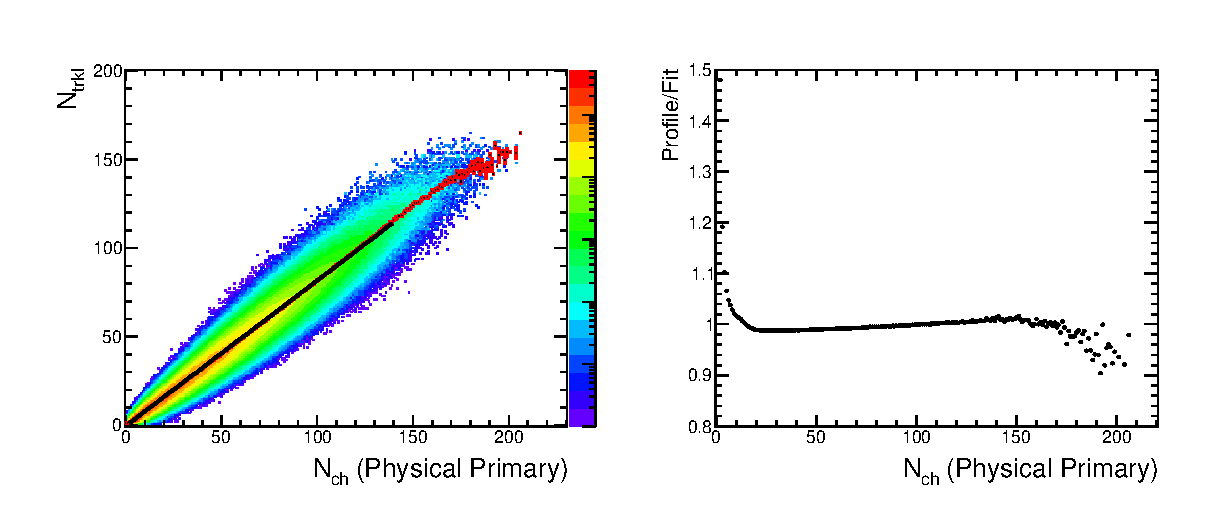
\includegraphics[width=1.\textwidth]{FigCap6/NtrklVsNchPhysPrimWithNtrklsReweight17f2a.eps}
 \caption{$\Ntrkl$ vs $\Nch$ distribution obtained for the 17f2a minimum bias production.}
 \label{fig:NtrklVsNch}
\end{figure}

\begin{figure}[h]
\centering
 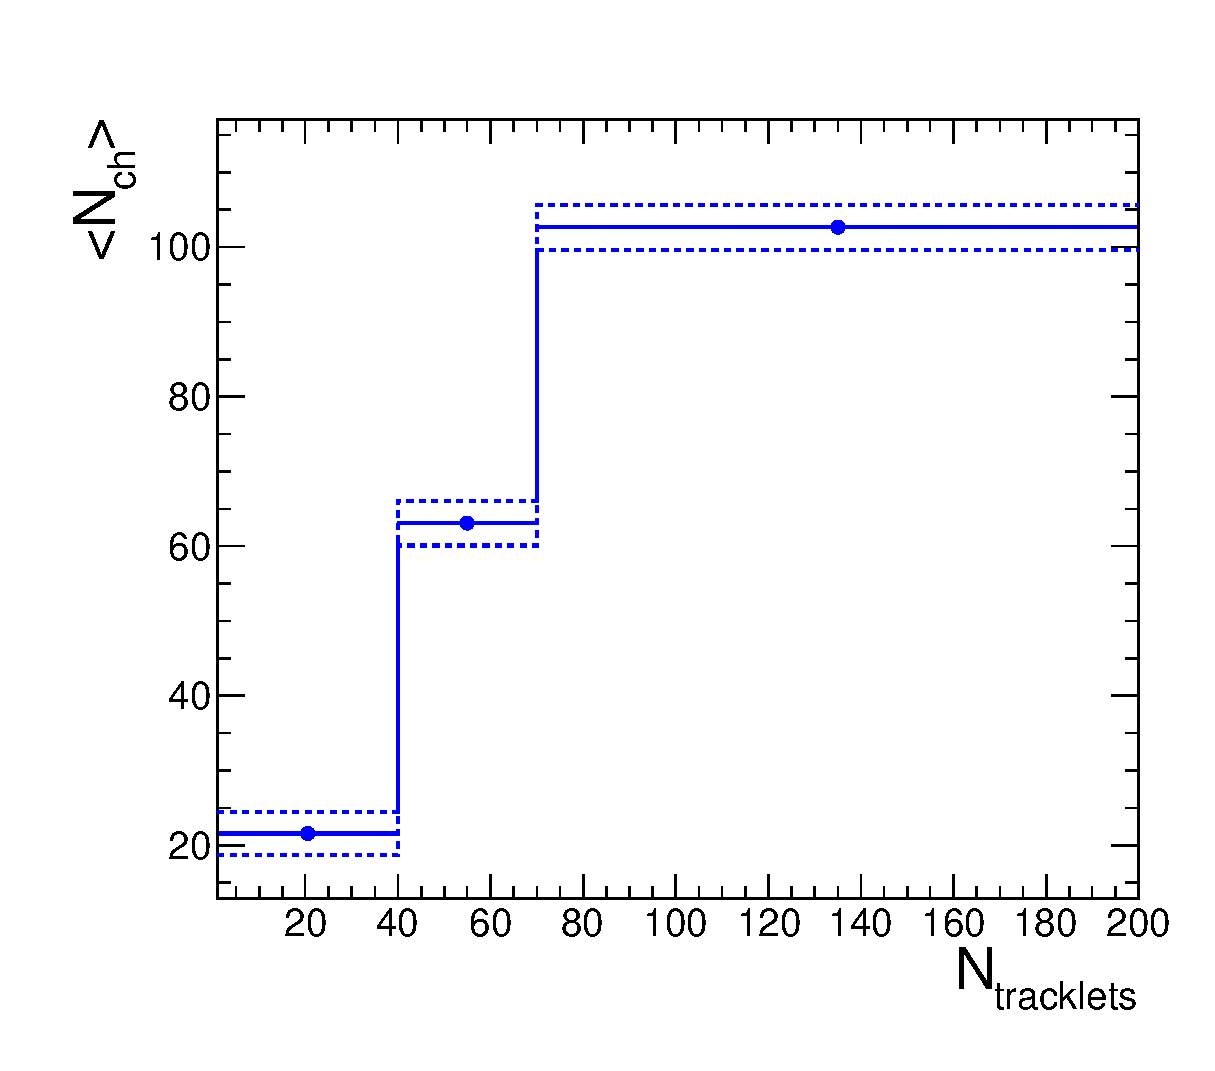
\includegraphics[width=.55\textwidth]{FigCap6/AverNchAndTotalSystUnc.eps}
 \caption{Average $\Nch$ values in the considered multiplicity classes, in the region $|\eta |< 1$. The lower and higher dashed lines represent the systematic uncertianties.}
 \label{fig:Nch}
\end{figure}

\subsubsection{Systematic uncertainty}
To estimate a systematic uncertainty on the evaluation of the average $\Nch$ value in the considered $\Ntrkl$ intervals, three different tests have been performed:
\begin{enumerate}
\item the conversion from $\Ntrkl$ to $\Nch$ was repeated with different MC generators 
\item the conversion from $\Ntrkl$ to $\Nch$ was repeated changing the assumption on the correlation (liear or not linear)
\item the conversion from $\Ntrkl$ to $\Nch$ was repeated with and without reweighting the $\Ntrkl$ vs. $\Nch$ histogram with the data-driven $\Ntrkl$ weights
\end{enumerate}

In particular, for the first point, the procedure was repeated considering the minimum-bias Monte Carlo productions LHC17f2a (EPOS generator) and LHC17f2b (DPMJET generator). Morevoer the result was also compared to the one obtained using the charm and beauty enriched MC production LHC17d2a, however the last one was not taken into account for the systematic uncertainties, since the forced decays of injected particles could induce a bias in the number of charged particles at mid rapidity. Fig.~\ref{fig:NchVsMCgenerator} shows the comparison of the average $\Nch$ obtained from the different MC productions.

\begin{figure}[htpb]
\centering
 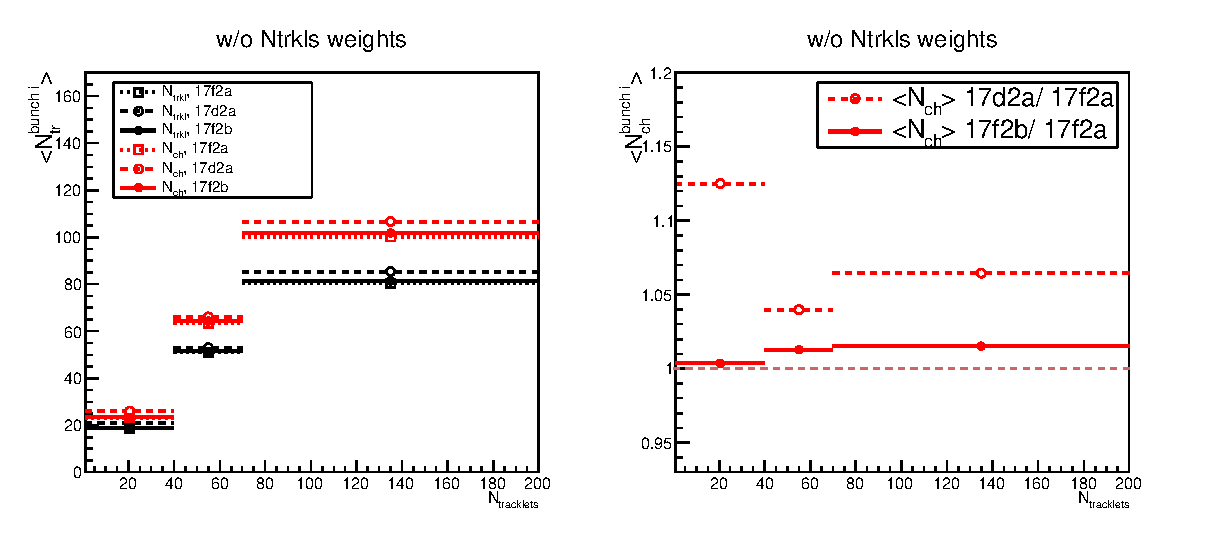
\includegraphics[width=.9\textwidth]{FigCap6/comparisonNtrkl_17f2b_17d2a_17f2a.eps}
 \caption{Left: Average $\Nch$ and $\Ntrkl$ values in the considered multiplicity classes, in the region $|\eta |< 1$, obtained from different MC productions. Right: ratio with respect to the default one (LHC172fa).}
 \label{fig:NchVsMCgenerator}
 \end{figure}

Considering the second source of uncertainty, the average $\Nch$ was extracted fitting the 2D histogram with a second order polynomial and considering the mean of the $\Nch$ distribution in the $\Ntrkl$ intervals considered in the analysis. This was done to test the possible non linear correlation between $\Ntrkl$ and $\Nch$, which is especially observed at low multiplicity, as shown in the right panle of Fig.~\ref{fig:NtrklVsNch}. In Fig.~\ref{fig:NchVsCorrHypo} the comparison of the average $\Nch$ obtained with the three different methods (linear fit, parabolic fit and mean of the $\Nch$ distribution) is shown.

\begin{figure}[htpb]
\centering
 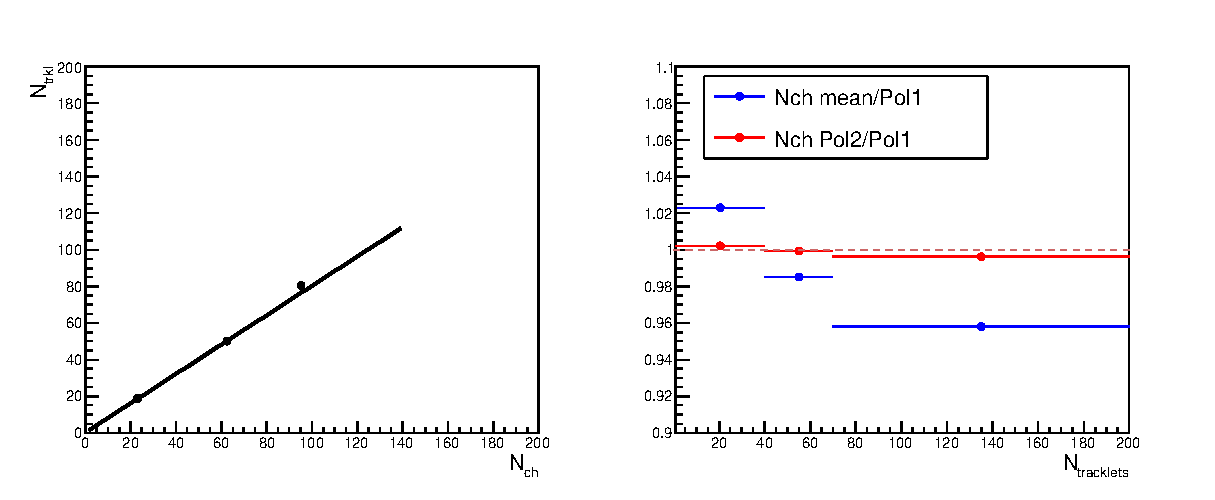
\includegraphics[width=.9\textwidth]{FigCap6/NchSystematics_linFit_17f2a}
 \caption{Comparison of the average $\Nch$ obtained with the three different methods (linear fit, parabolic fit and mean of the $\Nch$ distribution).}
 \label{fig:NchVsCorrHypo}
 \end{figure}

Finally, the average $\Nch$ was obtained without the data-driven $\Ntrkl$ weights and applying the weights obtained considering all the selected events, insted of the events that have at least a $\Dzero$ candidate in the correct mass range. This test is shown in Fig.~\ref{fig:NchVsNtrklWithWOweights}.

\begin{figure}[htpb]
\centering
 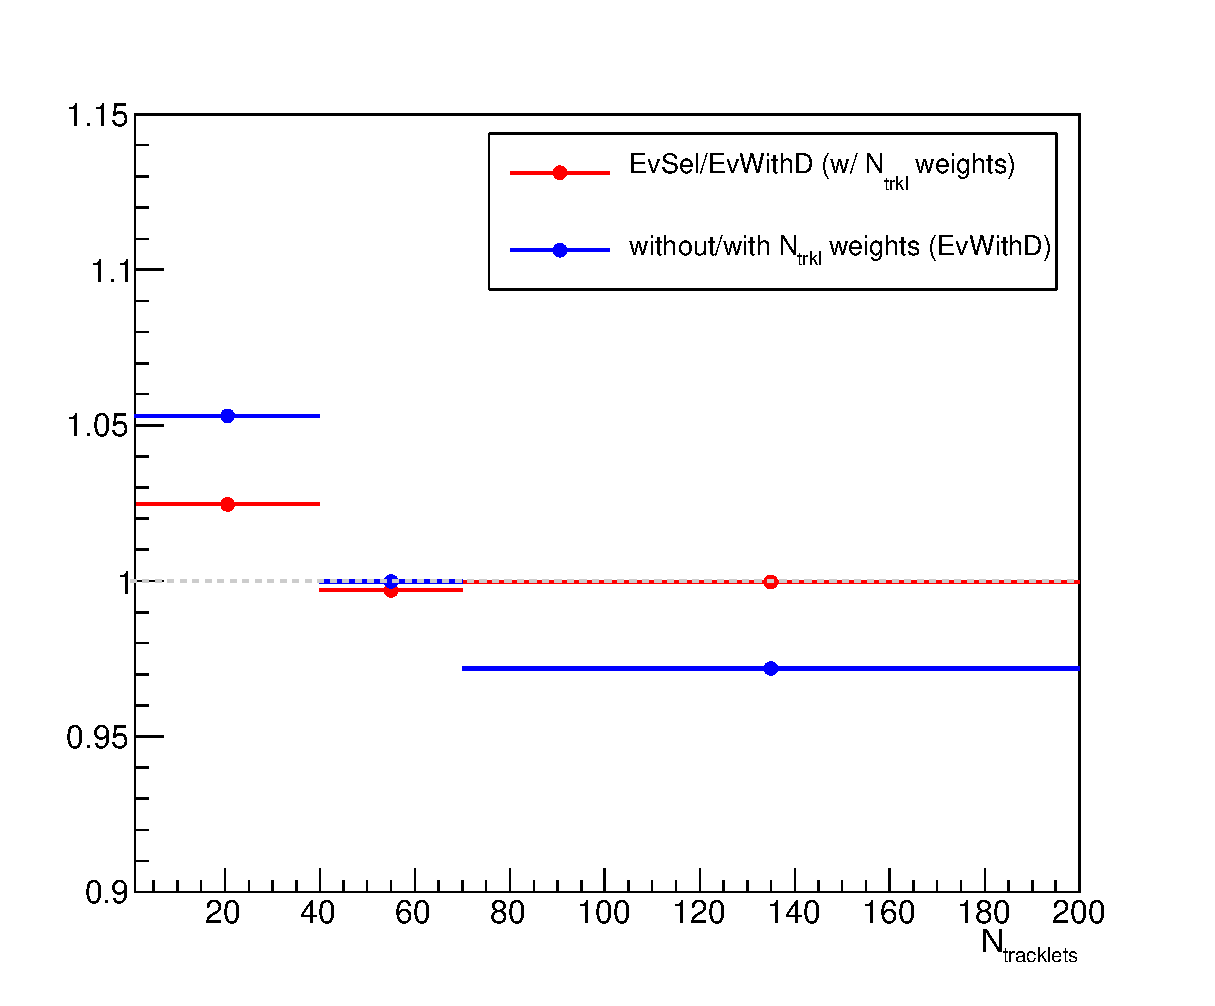
\includegraphics[width=.7\textwidth]{FigCap6/NchSystematics_NtrklWeights_17f2a.eps}
 \caption{Comparison of the average $\Nch$ obtained with and without data-driven $\Ntrkl$ weights.}
 \label{fig:NchVsNtrklWithWOweights}
 \end{figure}

Finally, the three sources of uncertainties have been considered as uncorrelated, and therefore summed in quadrature. The final result is shown in Fig.~\ref{fig:Nc}, where $\averNch$ in $|\eta|<1$ is shown with the corresponding systematic uncertainties.


\subsection{$\Ds/\Dplus$-meson yield ratios vs multiplicity }
The ratios of $\Ds/\Dplus$-meson yields are shown in Fig.~\ref{fig:DsDplusRatios} as a function of
the number of primary charged particles per unity of pseudorapidity, in the five $\pt$ intervals from 2 to 16 $\Gevc$.
The already measured ratios in pp collisions at $\sqrt{s}=$7 TeV and in Pb--Pb collisions at $\sqrt{s_{\rm NN}}=$ 5.02 TeV
(for the 0--10\%, 30--50\% and 60--100\% centrality classes, in the $\pt$ intervals where they are available) are also reported in the figure.
There is an hint of a non-flat trend between 2 $< \pt < 8~\Gevc$. The measured points were also
fitted with a linear function to have a quantitative indication of the slope, considering the statistical 
uncertainties only in the fit. The slopes from the linear fit on the pp, p--Pb and Pb--Pb points were found to be different from zero within 1$\sigma$ of the parameter error between 2 $< \pt < 8 ~\Gevc$, and between 4 $< \pt < 8 ~\Gevc$ for the
fit on pp and p--Pb measurements only (Fig.~\ref{fig:FitRatios}).

\begin{figure}[h!]
    \begin{center}
          \includegraphics[width=0.9\textwidth]{./FigCap6/DsOverDplusVsMult_pp7TeV_pPb5TeV_PbPb5TeV.pdf}
    \end{center}
    \caption{ $\Ds/\Dplus$-meson yield ratios as a function of the primary charged particles in $|\eta|<0.5$, in the different $\pt$ intervals from 2 to 16 $\Gevc$.}
    \label{fig:DsDplusRatios}
\end{figure}

\begin{figure}[h!]
    \begin{center}
          \includegraphics[width=0.9\textwidth]{./FigCap6/Fit_DsOverDplusVsMult_pp7TeV_pPb5TeV_PbPb5TeV.pdf}
    \end{center}
    \caption{Linear fit on $\Ds/\Dplus$ ratios as a function of the primary charged particles, in the different $\pt$ intervals from 2 to 16 $\Gevc$. The slope of the pol1 is reported in each pad, for the fits made only on the pp and p--Pb measurements or on
    all the pp, p--Pb and Pb--Pb points.}
    \label{fig:FitRatios}
\end{figure}





